%\cleardoublepage
%
\phantomsection
\chapter{State of the Art}
%
\label{cap:stateofart}
This chapter presents the state of the art concerning the areas which this thesis contribution is focused on. 

In the first part of the chapter, an overview on the Checkpoint/Restart technique is provided, with a brief summary of some of the most known technologies used to implement it.

The second part of the chapter will, instead, focus on the Run-Time Resource Management and its correlation with the resource allocation problem.

\section{Checkpoint/Restart}
\label{sec:criu}
\begin{figure}
    \centering
    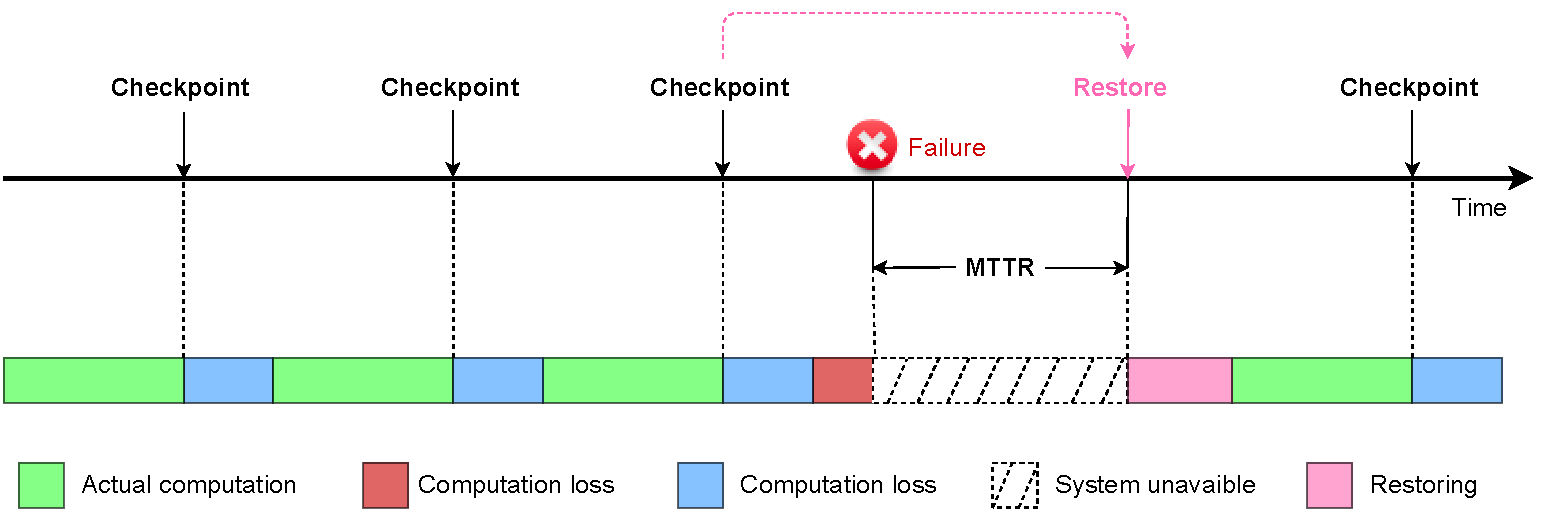
\includegraphics[width=\textwidth]{chk_rst.pdf}
    \caption{The Checkpoint/Restart approach.}
    \label{fig:chkrst}
\end{figure}
As anticipated in {\hyperref[cap:introduction]{Chapter 1}}, reliability is nowadays playing an increasingly fundamental role in HPC systems and, in this scenario, the importance of fault tolerance mechanisms is growing with the advancing of the computing potential of such systems. For this reason, many technique have been implemented to improve reliability and availability of parallel and  possibly distributed contexts: \emph{rollback-recovery} techniques are one of the most used solution for long running application.

\emph{Application Checkpointing} is the act of saving a snapshot of the state of a computation in order to be able, in case of failure, to resume it with the least possible computation loss. Walters et al., in \cite{app-checkpoint}, highlight that, from a high level perspective, three main steps are needed to perform a checkpoint:
\begin{enumerate}
    \item Interrupt the computation.
    \item Save the address space to a file.
    \item Save the register set to a file.
\end{enumerate}
\emph{Checkpoint/Restart (C/R)} is a widespread rollback-recovery technique which resorts to Application Checkpointing in order to enforce fault tolerance of computing systems. A summary of the approach provided by C/R is depicted in Figure~\ref{fig:chkrst}. C/R tools save the state (\emph{image}) of the processes in a non-volatile storage so that, when a system failure occurs, the image can be recovered and used to restart the execution from the saved checkpoint state.

When considering clusters of machines, each of which with a different failure rate, new problems arise. If a single application makes use of an entire cluster for its execution, synchronization among the machines is needed. Generally, C/R tools follow the three steps listed below \cite{reghenzani_2016}:
\begin{enumerate}
    \item Synchronization of the application processes execution to reach a global consistent state (\emph{sync}).
    \item Application execution state saving (\emph{checkpoint}).
    \item Application execution resuming (\emph{restart}).
\end{enumerate}
Depending on the level in which they operate, C/R tools are divided in four main categories and result transparent to the other layers \cite{app-checkpoint}:
\begin{description}
    \item[Hardware-level.] In this configuration, additional hardware is integrated with the processor to execute the checkpointing routine.
    \item[Kernel-level.] The operating system is in charge of the execution of the checkpointing code.
    \item[User-level.] An external library is linked to the program and is responsible for the checkpointing process.
    \item[Application-level.] The checkpointing code is inserted in the application code by the programmer.
\end{description}
At the time of writing, C/R routines are very expensive in terms of time stolen from the actual computation: the overall overhead  may reach over the 50\% of the total execution time \cite{6468485}.

In the years, several software tools implementing the Checkpoint/Restart mechanism have been distributed: an overview of some of the most known ones is provided below.

\begin{description}
    \item[Libckpt.] \verb|libckpt| \cite{260469} is a user-level library, developed in 1994 for UNIX system, then ported to a variety of kernels and operating systems. Checkpoints are performed by the tool using an incremental technique, i.e. when a checkpoint is taken, only the portion of the image that is changed since the last saved dump is stored. Additionally, copy-on-write, a mechanism used to optimize the copying of the main memory, is exploited in order to parallelize the execution of the application code and the writing in storage of the produced image. Checkpoints are executed periodically linking the library directly to the application at issue.
    \item[Berkeley Lab Checkpoint/Restart (BLCR).] BLCR \cite{duell2005design} is an open source software tool developed by the  Department  of  Computer  Science  of  the  Berkeley  Laboratory in 2003. Implemented as a Linux kernel module as well as a user-shared library, it supports both checkpointing of processes running on a single computers and parallel jobs running across multiple nodes of a Linux cluster, such as \emph{Message Passing Interface (MPI)} applications. It uses a non-blocking \verb|ioctl|, a special system call supported by UNIX and UNIX-like systems for device-specific input/output operations, to initiate the checkpointing in order to allow other computation to be performed. BLCR was improved and maintained until 2013 \cite{reghenzani_2016}.
    \item[MultiThreaded CheckPointing (MTCP).] MTCP \cite{Rieker06transparentuser-level} is a  checkpoint tool for \emph{Linux} operating system, which provides periodical checkpoints. It is composed of two binaries \verb|mtcp.so| and \verb|mtcp_restart|. The first one periodically saves the state of all threads, memory and list of open files to a checkpoint file. The second one reconstructs, on demand, the process from those files. It uses a wrapper function around \verb|clone| Linux function to capture the location of the stack (an argument of clone), and therefore specify the location of the stack on restart. It sets up data structures able to track creation and deletion of threads in an application and spawns a \emph{checkpointing control thread} to signal the application threads when a checkpoint needs to be performed. 
    \item[Distributed MultiThreaded CheckPointing (DMTCP).] DMTCP \\\cite{5161063} is a transparent user-level checkpointing package for distributed applications, extending MTCP. It does not depend on a specific message passing library nor on kernel modification. Designed for clusters of computers, it uses a \emph{coordinated checkpointing} method, which forces the suspension of all processes and threads in the cluster when a checkpoint occurs. It has been demonstrated scalable in the number of nodes of the cluster.
    \item[Checkpoint/Restore In Userspace (CRIU).] CRIU \cite{criu} is a software tool for Linux Operating Systems providing several features, starting from the basic Checkpoint/Restart functionality arriving at the more complex live migration and remote debugging \cite{reghenzani_2016}. It provides three different types of interfaces to use its services: \emph{Command Line Interface (CLI)}, \emph{Remote Procedure Call (RPC)}, which uses \emph{Google Protocol Buffers} to encode its calls, and a \emph{C Application Program Interface (C API)} called \verb|libcriu|, a wrapper around the RPC which facilitates the integration with C code. In order to perform a checkpoint, CRIU inject \emph{parasite code} in the process tree, it collects processes resources and save them, and, finally, it kills the application or remote the injected code to continue the execution \cite{reghenzani_2016}. CRIU is supported by the BarbequeRTRM\footnote{An overview upon the BarbequeRTRM is provided in {\hyperref[cap:implementation]{Chapter 3}}.}, the framework the work presented by this thesis have been integrated on.
\end{description}

Although checkpointing mechanisms play a fundamental role in the fault tolerance and availability of HPC systems, they might result insufficient without a proper logic behind the scheduling of the dumps. If CRIU only provides the user with a command through which a checkpoint gets launched, also a periodic checkpoint routine, as in the case of \verb|libckpt| and MTCP, is not ideal as a scheduling logic. Although such logic guarantees a maximum computation loss equal to the period length\footnote{Assuming a successful completion for each performed checkpoint.}, it does not take into account possible timing requirements of the specific application. Even if the period time might be a priori considered \emph{tolerable} as a worst-case computational loss, the possible variability of the checkpoint overhead itself cannot be managed directly. 

The work presented by this thesis tries to face the limits caused by the absence of a proper scheduling logic in CRIU, by implementing a dedicated checkpoint scheduler able to launch a checkpoint routine based on \emph{application-specific} performance and reliability requirements.

\subsection{Checkpoint/Restart and GPUs}
As already mentioned in {\hyperref[cap:introduction]{Chapter 1}}, in recent years, GPUs are playing an increasingly fundamental role in HPC systems. While supercomputers continue to scale in the number of GPUs, fault tolerance becomes a matter of major concern due to the presence of soft errors and the lack of error protection \cite{7056044}.

Ironically, while the need for transparent checkpointing of GPUs has grown in the last decade, the support for transparent checkpointing of GPUs has diminished \cite{10.5555/3433701.3433803}. In the years, many efforts have been made to develop C/R tools for GPUs, but all of them stopped working with the release of CUDA 4.0, in 2011, with \emph{Unified Virtual Addressing (UVA)} between host and GPU device, later refined, with CUDA 6.0, to \emph{Unified Virtual Memory (UVM)}. After these upgrades, all the previous checkpointing technologies became ineffective, since they created inconsistencies between host and GPU device address space during the restore of the checkpointed CUDA library and the associated allocated memory at their original address.

In recent years, two new tools, CRCUDA \cite{suzuki2016transparent} and CRUM \cite{8514890}, were released, trying to solve the problem through the use of separate proxy processes, however exposing limitations in terms of overhead and partial support for UVM. 

To the best of our knowledge, only a recent DMTCP plugin, CRAC \cite{10.5555/3433701.3433803}, have had successful results in the workaround of the UVM problem. However, although its source code is available \cite{dmtcp-crac}, the project is for the time being at an embryonic state. 

Due to the lack of dependable checkpointing technologies, the work proposed by this thesis does not include GPU applications checkpointing support, nevertheless, when such technologies will become available, an extension might be provided.

\section{The Resource Management problem}
Modern parallel computing architectures have broadened the boundaries of the HPC world, emerging in the Embedded Systems context too \cite{6322885}. On one hand, mobile systems are nowadays powerful enough to run computational intensive applications as 3D games and augmented reality. On the other hand, multi/many-core Systems-on-Chip allow embedded systems designers to choose among increasingly larger set of software solutions, without the need of changing hardware modules to implement a feature. Although this progress in systems capability results in a huge gain in terms of flexibility, cost and time to market, reliability and fault tolerance, it also comes with a non-trivial and diverse rationale behind the organization and management of the available resources. For instance, if, on one hand, mobile systems need to efficiently use computational resources in order to maximize batteries lifetime, on the other hand, mission-critical systems may need dynamic reallocation of tasks to minimize  thermal variations in the die. Furthermore, with the advancing of the technology progress, systems tend to enlarge their complexity and redundancy, making clear the need of a sensible resource management. In addition, the increasing impact of thermal concerns calls for a power and thermal aware resource management, resulting in a smart utilization of the processing and storing elements and in task scheduling methods which, making use of task migration and appropriate logic, take into consideration holistically and possibly at run time the diversity of performance and reliability issues. In this scenario,  Run-time Resource Managers (RTRM) take their place.

RTRMs act as system-wide arbiters to the resource contention and, by being aware of the run-time dynamism of resources and applications, allow the system to be more adaptive and re-configurable, considering possibly multiple objectives.

A powerful mean used to reach the above mentioned goal is to design resource allocation policies able to analyze the data coming from resources and applications run-time profiling, in order to properly bind them one to the others, using specific optimization criteria.

As widely discussed in the previous sections, reliability is becoming a more and more relevant concern in nowadays computing systems, enough to lead to the designing of several allocation policies whose main objective is to maximize the reliability level of the system.

Gottumukkala et al. \cite{4629245} designed a reliability-aware resource allocation policy for parallel programs, basing the prediction of the time between failure on the Weibull distribution. Ramani et al. \cite{7530840} proposed a power management technique aimed at, among other objectives, improve long term reliability of many-cores systems. Huang et al. \cite{5090632} presented a task allocation and scheduling technique for embedded Multi-Processor Systems on Chip (MPSoC) Platforms whose goal is to reduce the wear out of the hardware components.

The contribution of the work proposed by this thesis to the reliability management problem consists in the design and implementation of a resource allocation policy aimed at optimizing the reliability-performance trade off. This objective is reached through a periodical monitoring of reliability parameters of the available computing resources, which is used as an input for a smart binding to the running applications. The used approach not only improves the reliability of the applications, but also aims to slow down the aging of the hardware components, all of it with an as small as possible performance loss.